% Compile with XeLaTeX or LuaLaTeX (Overleaf: Menu > Compiler > XeLaTeX).
\documentclass[10pt,twocolumn,letterpaper]{article}
\usepackage[top=0.95in,bottom=0.9in,left=0.8in,right=0.8in,columnsep=0.28in,headheight=14pt,footskip=24pt]{geometry}
\usepackage{fontspec}
\setmainfont{TeX Gyre Pagella}
\usepackage{amsmath,amssymb}
\usepackage{graphicx}
\usepackage{booktabs,array}
\usepackage{xcolor}
\usepackage{titlesec}
\usepackage{fancyhdr}
\usepackage{lastpage}
\renewcommand{\topfraction}{0.92}
\renewcommand{\dbltopfraction}{0.92}
\renewcommand{\textfraction}{0.08}
\renewcommand{\floatpagefraction}{0.7}
\renewcommand{\dblfloatpagefraction}{0.7}
\setcounter{topnumber}{3}
\setcounter{dbltopnumber}{3}
\setcounter{totalnumber}{5}
\usepackage{caption}
\usepackage{enumitem}
\usepackage{url}
\usepackage{microtype}
\usepackage[hidelinks]{hyperref}
\urlstyle{same}
\sloppy
\setlength{\parindent}{0pt}
\setlength{\parskip}{3.5pt}
\renewcommand{\baselinestretch}{1.05}

% headings: "1 | Introduction" as in the Wiley journal layout
\titleformat{\section}{\bfseries\fontsize{11}{13}\selectfont}{\thesection\hspace{0.45em}|\hspace{0.45em}}{0pt}{}
\titleformat{\subsection}{\bfseries\fontsize{9.5}{11.5}\selectfont}{\thesubsection\hspace{0.45em}|\hspace{0.45em}}{0pt}{}
\titlespacing*{\section}{0pt}{10pt}{4pt}
\titlespacing*{\subsection}{0pt}{6pt}{3pt}

% captions: "FIGURE 1 | text"
\renewcommand{\figurename}{FIGURE}
\renewcommand{\tablename}{TABLE}
\DeclareCaptionLabelSeparator{bar}{\hspace{0.4em}|\hspace{0.4em}}
\captionsetup{font=footnotesize,labelfont=bf,labelsep=bar,justification=raggedright,singlelinecheck=false,skip=4pt}

% header and footer
\pagestyle{fancy}
\fancyhf{}
\fancyhead[L]{\colorbox{black!12}{\textit{\textbf{\small\ Systems Engineering\ }}}}
\fancyfoot[L]{\footnotesize\itshape MBSE framework for auxetic bone screws}
\fancyfoot[R]{\footnotesize\thepage\ of \pageref{LastPage}}
\renewcommand{\headrulewidth}{0pt}
\renewcommand{\footrulewidth}{0.4pt}
\fancypagestyle{plain}{\fancyhf{}\fancyfoot[L]{\footnotesize\itshape MBSE framework for auxetic bone screws}\fancyfoot[R]{\footnotesize\thepage\ of \pageref{LastPage}}\renewcommand{\headrulewidth}{0pt}\renewcommand{\footrulewidth}{0.4pt}}

\setlist[itemize]{leftmargin=1.1em,itemsep=1.5pt,topsep=2pt,parsep=0pt}
\setlength{\tabcolsep}{3pt}
\renewcommand{\arraystretch}{1.12}

\begin{document}

\twocolumn[{%
\vspace*{-4pt}
{\noindent\rule[-2pt]{2.5pt}{11pt}\hspace{5pt}{\small\bfseries RESEARCH ARTICLE}\par}
\vspace{8pt}
{\raggedright\fontsize{21}{25}\selectfont\bfseries A Model-Based Systems Engineering Framework for Requirements-Driven Design and Verification of Auxetic Bone Screws\par}
\vspace{8pt}
{\raggedright\textbf{G Mohammad Afzal}\\{\small\color{black!65} Roll No. ME23B2014}\par}
\vspace{8pt}
\noindent\colorbox{black!8}{\parbox{\dimexpr\textwidth-2\fboxsep}{\small\textbf{ABSTRACT}\\[2pt]Auxetic bone screws have a porous core with a negative Poisson's ratio, so the core widens when the screw is pulled, which should improve grip. The same compliant core, though, creates a stiffness step where it meets the solid head, and fatigue life is predicted to be shortest at that junction. We call this the auxetic transition paradox. Screw designs are developed through separate CAD and finite element studies with no formal link to requirements. This paper presents a model-based systems engineering (MBSE) framework for an auxetic screw. SysML models are combined with a V-model, the screw is split into four subsystems, and a generative design step builds the porous core from the requirements. Three unit cells (re-entrant chevron AS1, re-entrant hourglass AS2 and a hexagonal control NS) were generated at equal strut thickness and analysed in COMSOL Multiphysics 6.2 under a 0.20 mm tensile displacement. On the finest of five meshes the axial reaction force was 3,096 N for AS1, 2,382 N for AS2 and 958 N for NS, and the order never changed. Peak stress did not converge and was used only to rank. A graded variant of AS2, made by changing one parameter, lowered the stress next to the head by about 19\% but moved the hot spot into the graded zone. All eight requirements are linked to verification cases, yet the evidence is simulated only, and two requirements stay open. The trace exposed a weak acceptance criterion and a missing check at the collar neck.}}\par
\vspace{6pt}
{\small\textbf{Keywords:} model-based systems engineering | SysML | generative design | auxetic metamaterials | bone screw | requirements traceability | finite element analysis\par}
\vspace{6pt}
}]


\section{Introduction}
\subsection{Fixation failure and the auxetic idea}
Bone screws are among the most common implants in orthopaedic surgery. When they fail, the usual cause is that the screw loosens or pulls out of the bone. Barnett et al. report that such migration or pullout accounts for roughly 10\% of fracture-fixation failures [1]. Bone cement can improve grip, but it brings its own complications [2]. Auxetic structures offer another route. A material with a negative Poisson's ratio (NPR) gets wider when it is stretched [3--5]. If the core of a screw is built from auxetic cells, a pulling load should make the screw expand sideways and press harder against the bone around it.

Yao et al. placed six auxetic cells (A1 to A6) into screw bodies (AS1 to AS6) and compared them with a non-auxetic screw (NS) in finite element pullout models. AS2 gave the stiffest and strongest response and the highest pullout force, 1,185.93 N in high-density bone [2]. In a follow-up on pedicle screws, stronger auxeticity helped only when the elastic modulus was held equal, and the right modulus was a precondition for good performance [6]. Barnett et al. tested unthreaded polymer fasteners in bone analogue. A rotating-squares design carried 2.5 times the pullout load of its non-auxetic control, and the authors linked this to its low axial stiffness [1]. So stiffness and fixation do not move together in any simple way, and that shapes how we read our own results in Section 5.

\subsection{The auxetic transition paradox}
The feature that makes an auxetic screw attractive also weakens it. The porous, compliant core gives the radial expansion, but it also makes the step between the solid head and the porous shaft the most fatigue-critical part of the screw. We call this the auxetic transition paradox. Wang et al. found that re-entrant auxetic screws had a tensile fatigue strength about 43\% lower than non-auxetic screws of the same 51\% porosity, although bone grew into them better [7]. Huang et al. studied the stress concentration in the auxetic porous screw [8]. In a later multiaxial simulation of ankle fusion (tibiotalocalcaneal arthrodesis), they estimated about 46,400 cycles to failure for the auxetic screw and 1,820,000 for the non-auxetic one, a 97.5\% reduction. The shortest life and the highest principal stress were next to the screw cap, where the screw meets the fixation plate, and the authors recommended redesigning that region [9]. These are simulated lives and not clinical failures, but they are the specific evidence that led us to give the head-to-shaft junction its own subsystem.

\subsection{Gap and research questions}
The auxetic screw studies we reviewed handle design through separate unit-cell, finite element and mechanical studies [2, 6, 7, 9]. We found no published work that links stakeholder needs, requirements, architecture, CAD and verification for an auxetic screw in one maintained model. In MBSE, a maintained system model is the authoritative source of requirements, architecture and verification links [10, 11]. It is a natural way to close that gap. The paper asks three questions.

\begin{itemize}
\item \textbf{RQ1.} Can SysML requirements and a V-model be used to drive the geometry of a porous auxetic implant directly, so that design changes follow from model parameters?
\item \textbf{RQ2.} What can a simulation-only verification say about the requirements, and what can it not say?
\item \textbf{RQ3.} Does the explicit trace help to find and fix weak requirements early?
\end{itemize}
\subsection{Contributions and scope}
The paper makes four contributions. First, it gives a SysML and V-model framework that connects stakeholder needs, requirements, architecture blocks, CAD parameters and finite element cases for an auxetic bone screw. Second, it proposes a four-subsystem architecture in which the head-to-shaft transition is a verifiable subsystem of its own. Third, it adds a requirements-driven generative design step that partitions the design space, calibrates each topology to a target porosity and grades the strut thickness along the axis to test the transition collar. Fourth, it reports a simulation study of three unit cells with a mesh-convergence check, and says plainly which requirements the evidence supports.

The scope is limited on purpose. The work is computational. There is no bone in the model and no physical or fatigue test, so all conclusions are about the isolated screw.


\section{Background}
\subsection{Auxetic structures for fixation}
Auxetic behaviour comes from cell geometry, not from the base material. Cellular auxetics are usually grouped into re-entrant, chiral, rotating-rigid and perforated-sheet families [4]. They have been proposed for joint, spinal and trauma surgery [5]. For screws, the relevant designs are the re-entrant families studied in [2, 6, 7]. We use the naming of Yao et al.: A1, A2 and N for the planar cells, and AS1, AS2 and NS for the screws built from them. Whether our A1 and A2 geometries match the original cells exactly has not been checked.

\subsection{MBSE and SysML}
MBSE puts a system model at the centre of development. The model supports specification, design, verification and configuration control, and it keeps the trace between them [10]. Its processes fit ISO/IEC/IEEE 15288:2023 and the INCOSE Systems Engineering Handbook [11, 12]. SysML is the standard modelling language [13], and version 2.0 was adopted by the Object Management Group in 2025 [14]. Our diagrams were drawn in Visual Paradigm. The constructs we use (requirements, blocks, ports, activities, and the satisfy, verify and deriveReqt relationships) exist in both SysML versions.

\subsection{Design controls and simulation credibility}
Design controls for medical devices are set out in ISO 13485:2016, clause 7.3 [15]. In the United States, the Quality Management System Regulation (QMSR) took effect on 2 February 2026. It incorporates ISO 13485 into 21 CFR Part 820 and replaces the older design-control section 820.30 [16, 17]. We therefore use ISO 13485 clause 7.3 as the design-control reference, together with ISO 14971 for risk management [18]. For computational evidence, ASME V\&V 40 and the FDA guidance of 2023 say that the credibility a model needs depends on how much the decision relies on it and how bad a wrong decision would be. They separate code verification, calculation verification and validation [19, 20]. We use these ideas in Section 5 to say what our simulations can and cannot support.


\section{MBSE Framework}
\subsection{V-model decomposition}
Figure 1 shows the framework. The left side of the V goes from stakeholder needs (L1: surgeon, patient, manufacturer) to system requirements (L2), functional architecture (L3), subsystem design (L4) and parametric CAD (L5). The right side goes back up: unit-cell checks (R5), subsystem checks (R4), functional checks (R3), system checks (R2) and clinical validation (R1). Dashed links show two-way traceability. At the bottom of the V, a Python script in Fusion 360 builds the CAD and a Java script drives COMSOL in batch mode. In this paper levels R5 to R2 are addressed by simulation, in part. R1, a bone-block pullout test, is planned and has not been done.

\begin{figure*}[!t]
\centering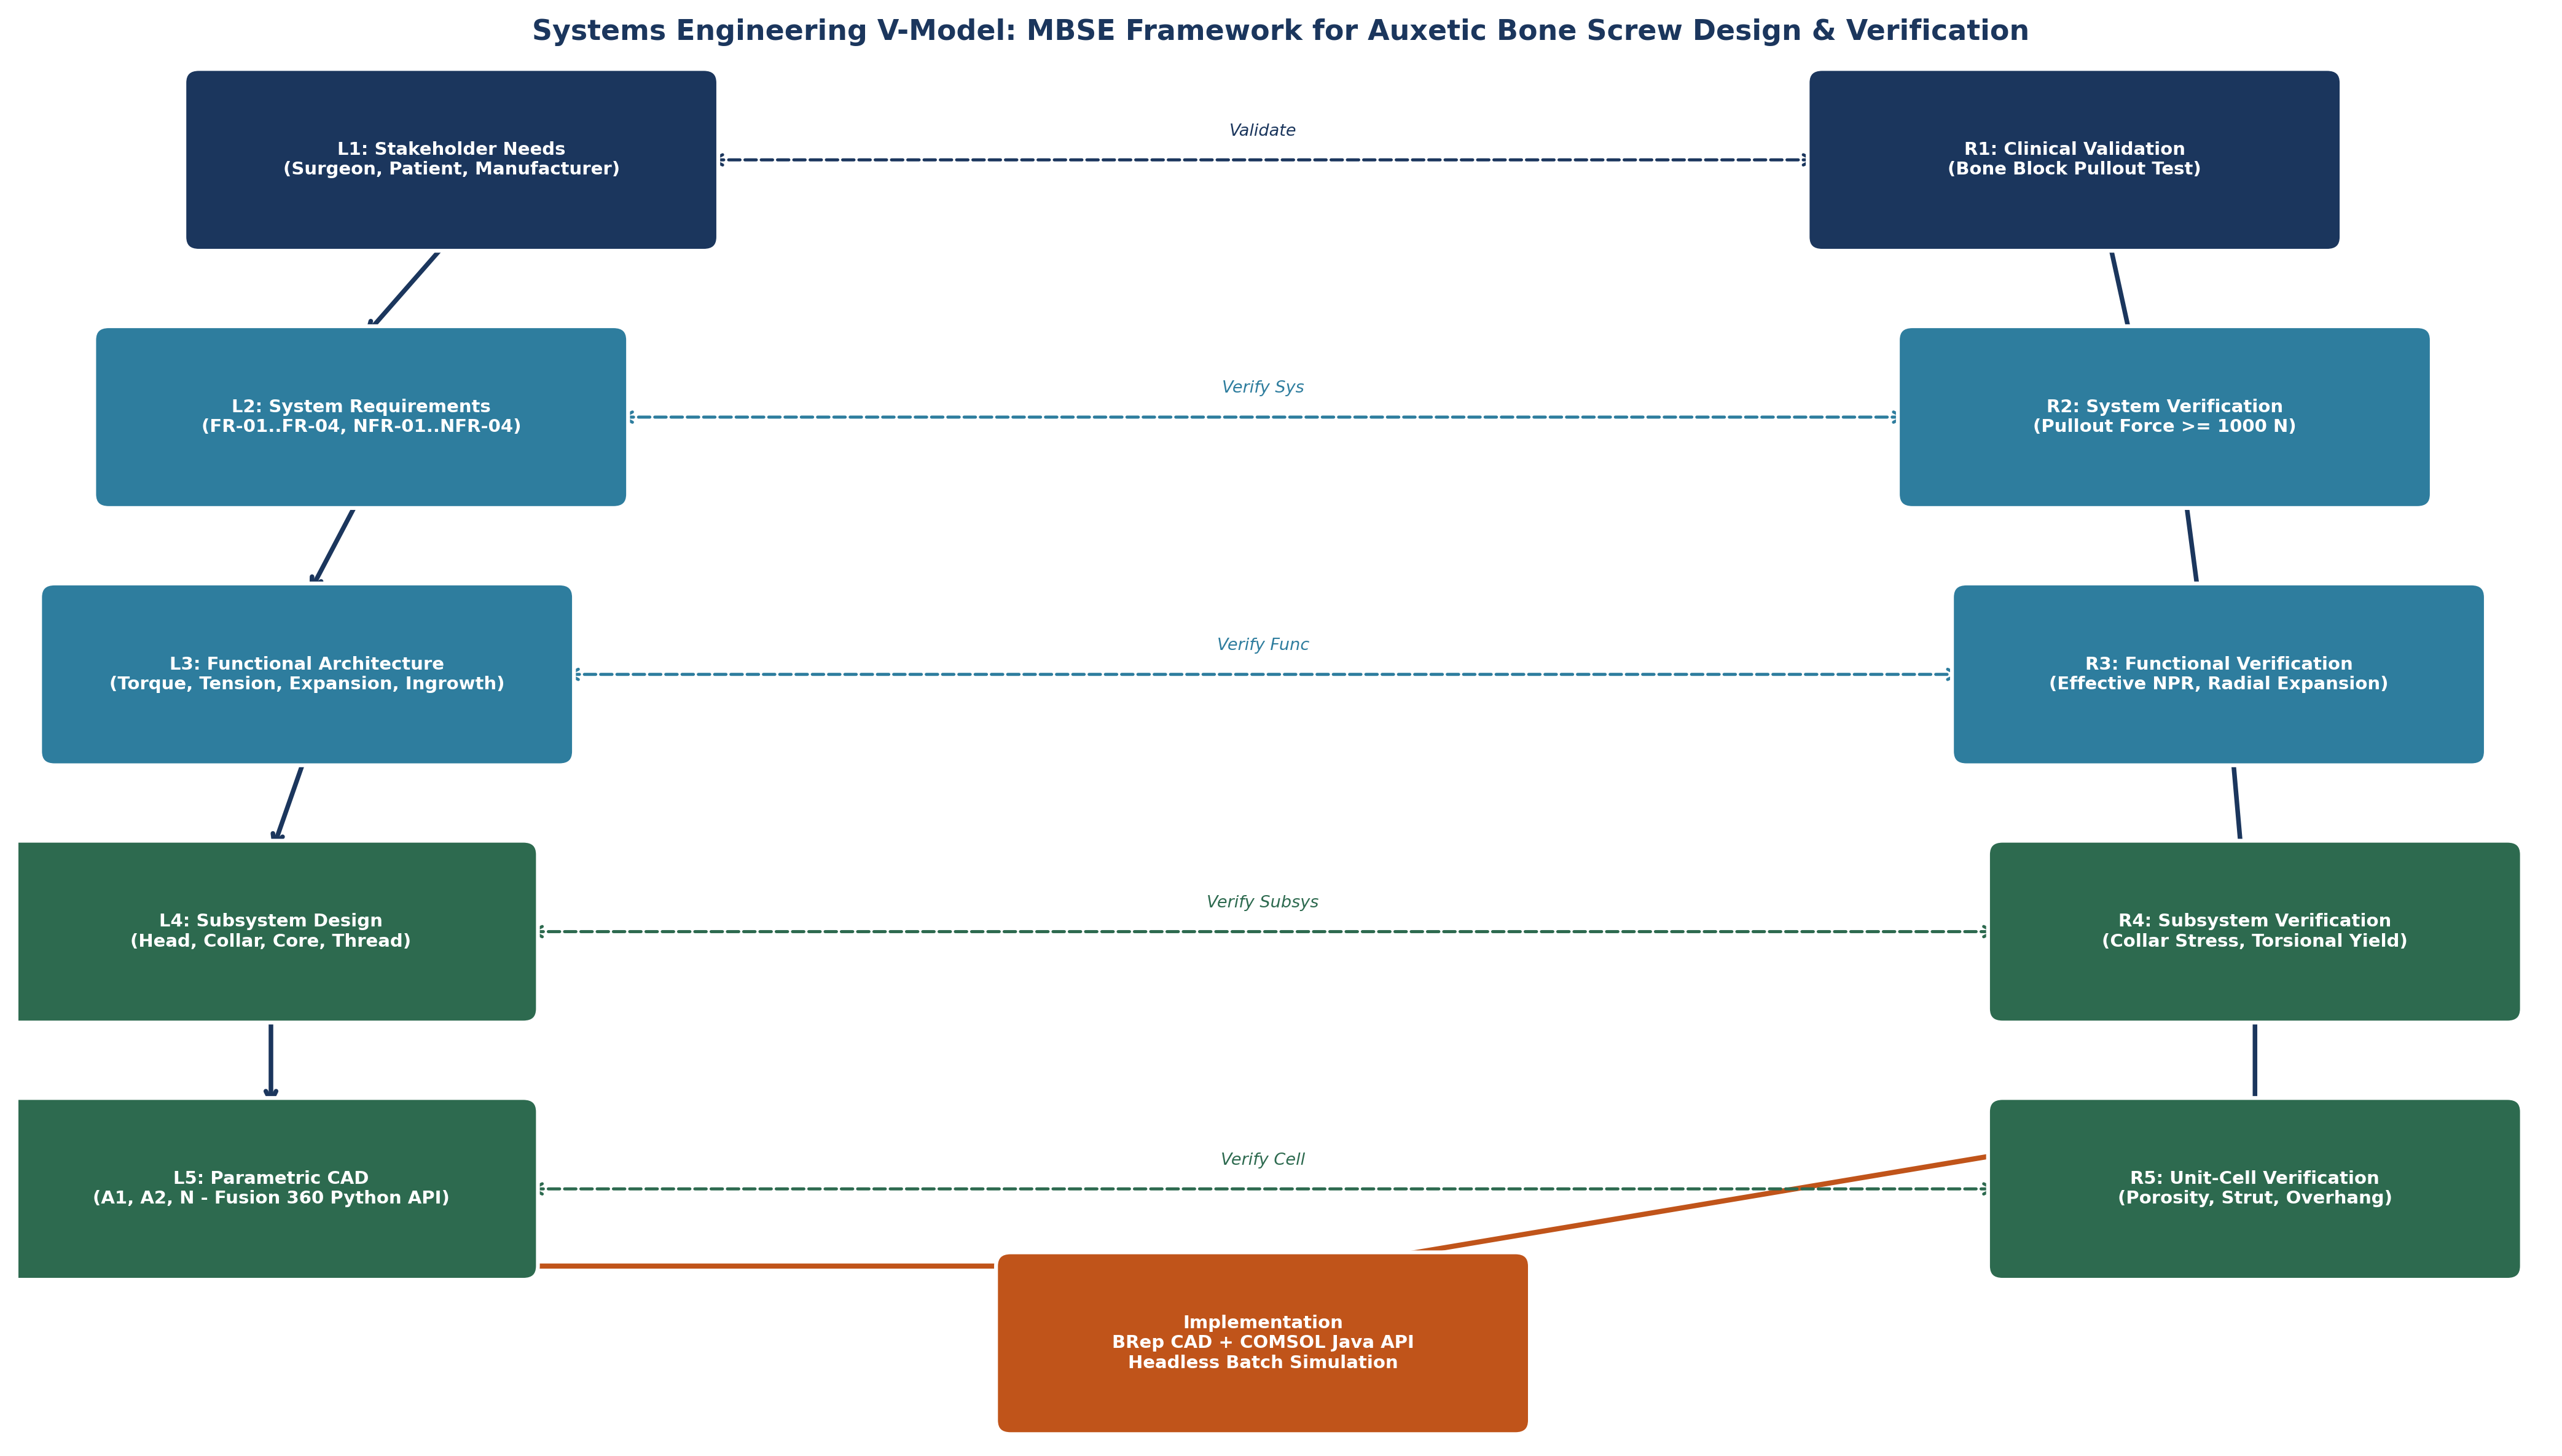
\includegraphics[width=\textwidth]{figures/v_model_diagram.png}
\caption{V-model of the framework. The left branch (L1 to L5) runs from needs to parametric CAD and the right branch (R5 to R1) from unit-cell checks to validation. Only R5 to R2 are covered here, by simulation.}
\end{figure*}
\subsection{SysML model suite}
Four linked diagrams make up the model baseline (Figure 2). The requirements diagram holds the deriveReqt hierarchy. The block definition diagram shows the four subsystems. The internal block diagram shows the torque, load and kinematic ports between them. The activity diagram follows insertion and tensile expansion across four lanes: surgeon, head and collar, host bone, and porous core. Satisfy, verify and deriveReqt relationships connect the diagrams.

\begin{figure*}[!t]
\centering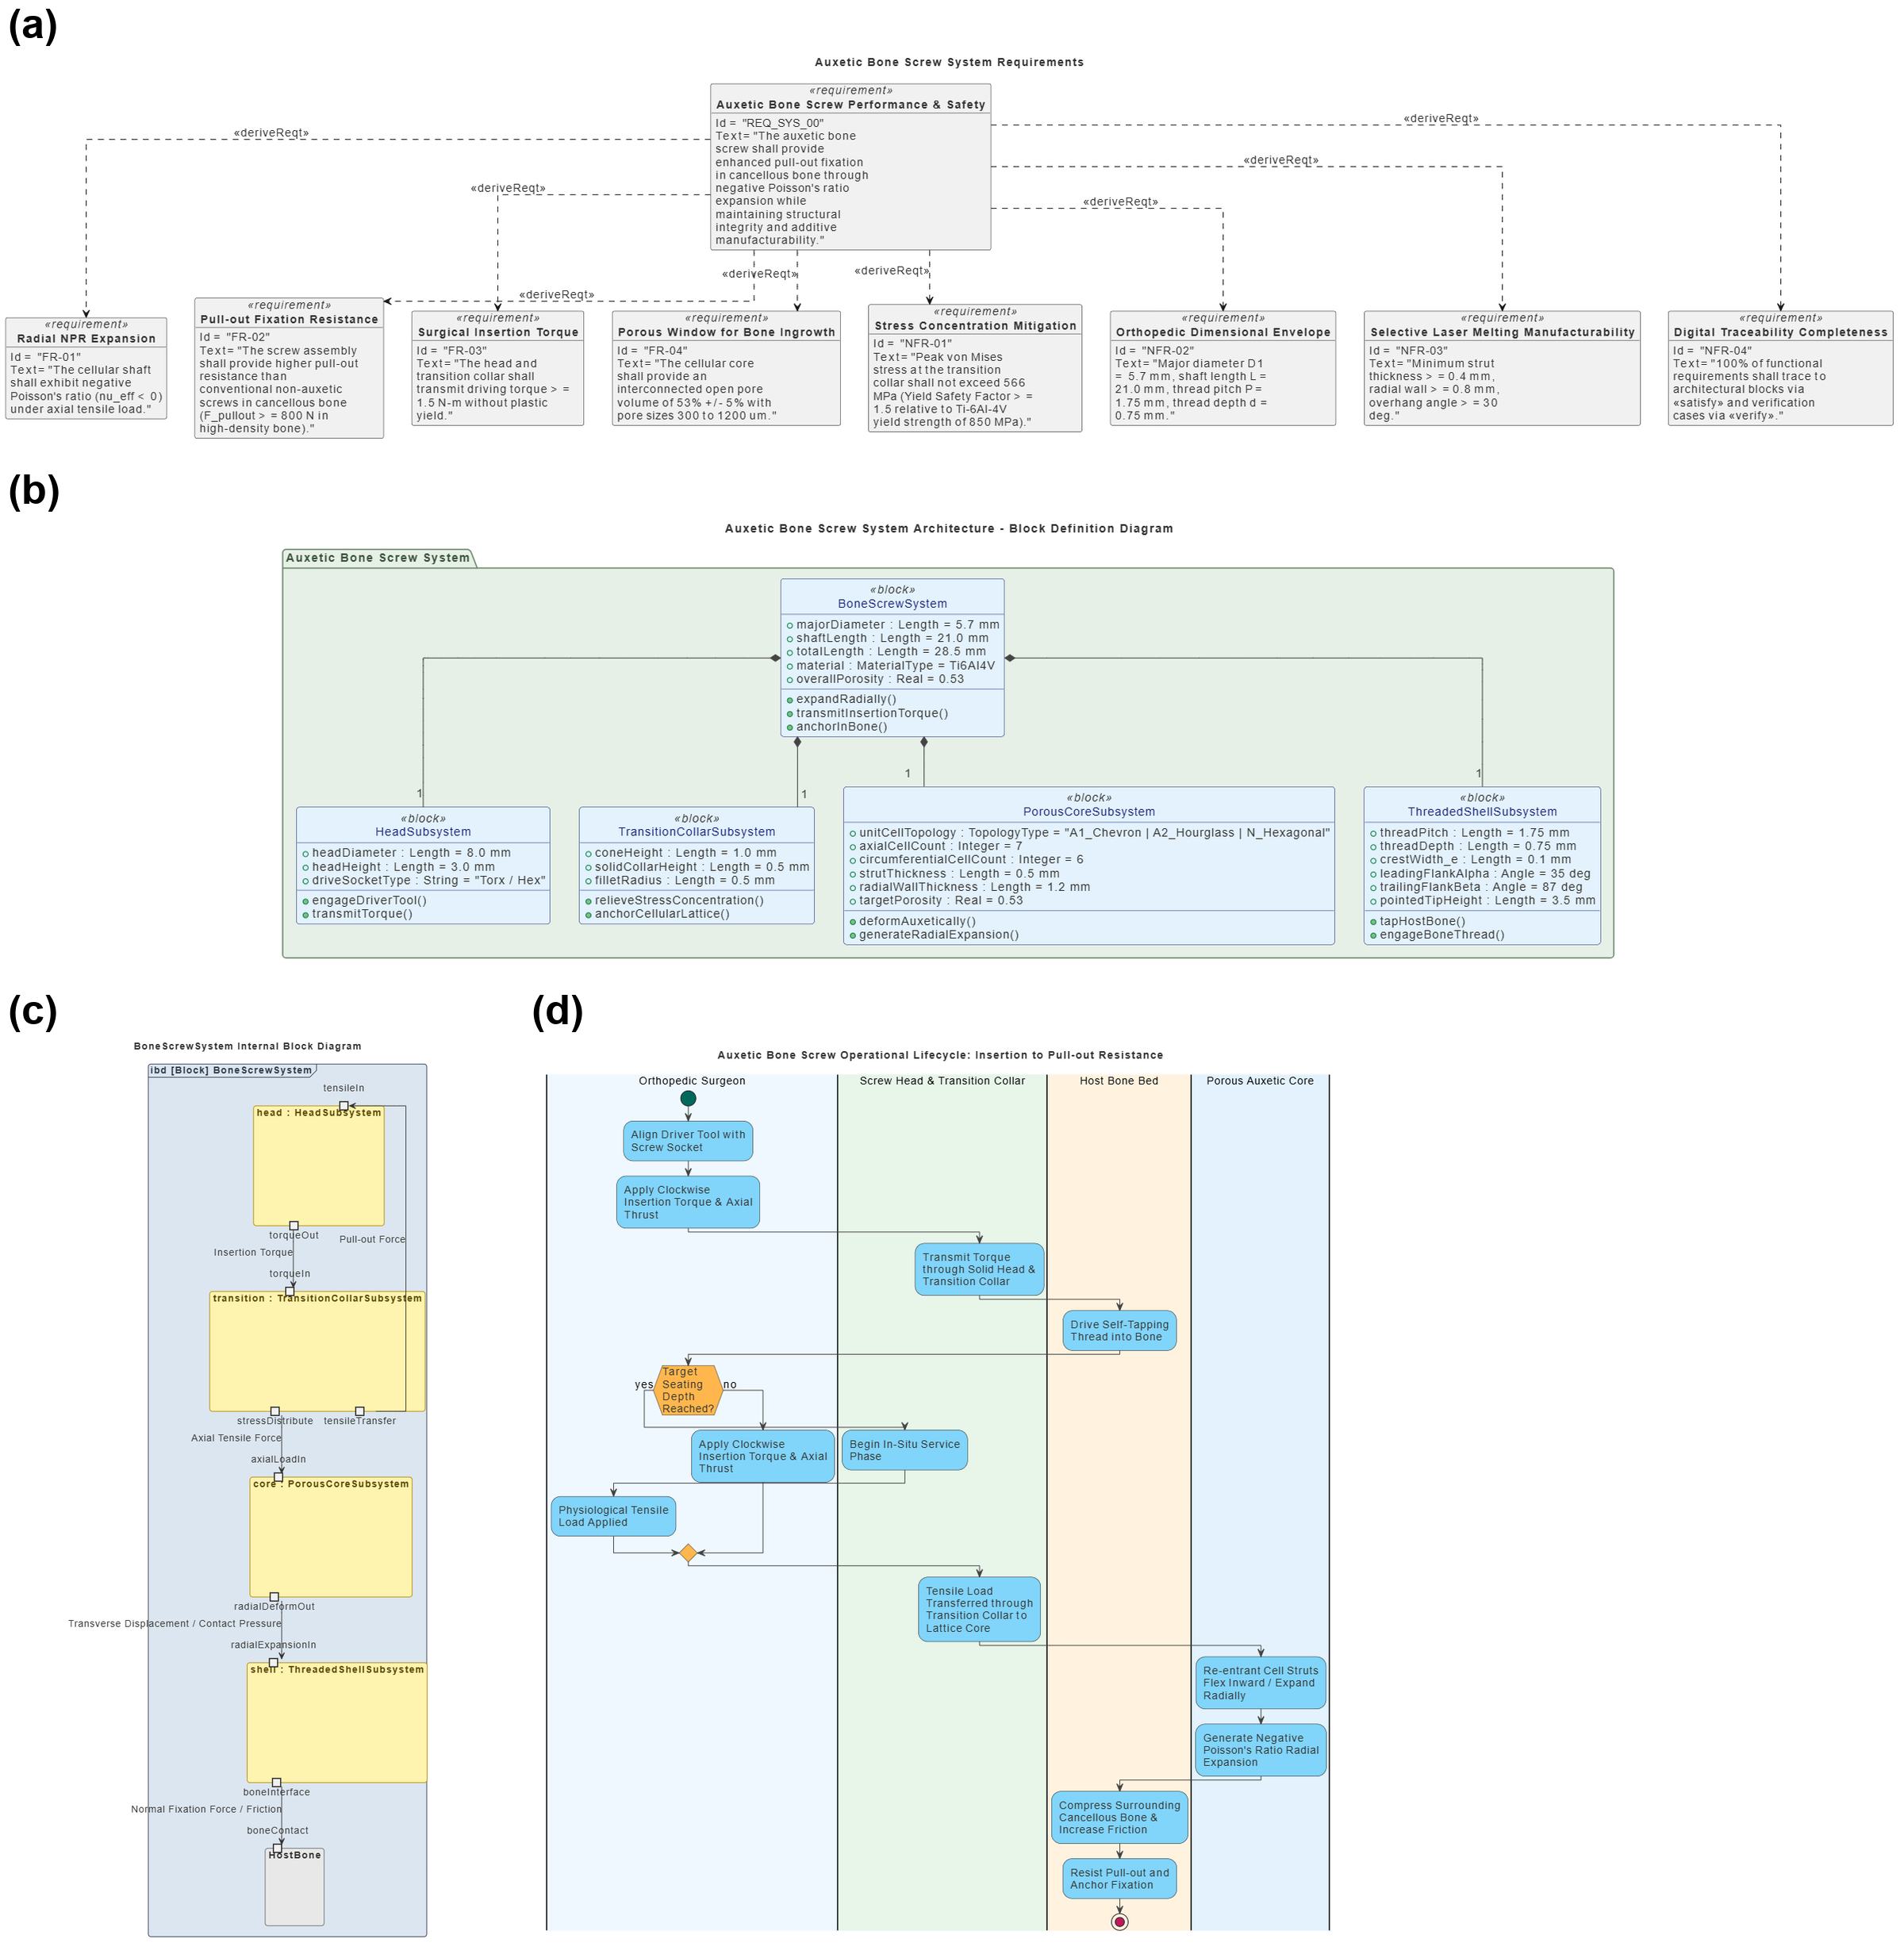
\includegraphics[width=\textwidth]{figures/sysml_composite.png}
\caption{SysML baseline: (a) requirements diagram, (b) block definition diagram, (c) internal block diagram, (d) activity diagram. Text is small at print size and legible in the electronic file.}
\end{figure*}

\section{Requirements, Architecture and Generative Design}
\subsection{Stakeholder needs and requirements}
Five stakeholder needs drive the design. The surgeon needs better primary fixation in osteoporotic bone without cement (SN-01) and standard driver engagement with predictable torque transfer (SN-02). The patient needs protection against fatigue fracture at the screw neck (SN-03). The manufacturer needs a design that can be printed by selective laser melting (SLM) with struts of at least 0.40 mm and open channels to remove powder (SN-04). The regulator needs design-control traceability under ISO 13485 clause 7.3 (SN-05). Table 1 lists the eight requirements derived from these needs.

\begin{table*}[!t]
\caption{Requirements derived from the stakeholder needs (FR = functional, NFR = non-functional).}
\centering\fontsize{8}{9.6}\selectfont
\begin{tabular}{>{\raggedright\arraybackslash}p{\dimexpr(\linewidth-10\tabcolsep)*112/1000\relax}>{\raggedright\arraybackslash}p{\dimexpr(\linewidth-10\tabcolsep)*272/1000\relax}>{\raggedright\arraybackslash}p{\dimexpr(\linewidth-10\tabcolsep)*320/1000\relax}>{\centering\arraybackslash}p{\dimexpr(\linewidth-10\tabcolsep)*88/1000\relax}>{\centering\arraybackslash}p{\dimexpr(\linewidth-10\tabcolsep)*208/1000\relax}}
\toprule
\textbf{ID} & \textbf{Requirement} & \textbf{Acceptance criterion} & \textbf{Need} & \textbf{Subsystem} \\
\midrule
\textbf{FR-01} & Negative Poisson's ratio & $\nu_{\mathrm{eff}}$ < 0 & SN-01 & S3 Core \\
\textbf{FR-02} & Tensile fixation & $F_{y}$ $\geq$ 1,000 N at $U_{y}$ = 0.20 mm & SN-01 & Whole screw \\
\textbf{FR-03} & Insertion torque transfer & $\tau$ $\geq$ 1.5 N$\cdot$m, $\sigma$ < $\sigma_{y}$ & SN-02 & S1 Head, S2 Collar \\
\textbf{FR-04} & Osseointegration porosity & 53.0\% $\pm$ 5.0\% & SN-01 & S3 Core \\
\textbf{NFR-01} & Stress relief at transition & Safety factor $\geq$ 1.5 at collar neck & SN-03 & S2 Collar \\
\textbf{NFR-02} & Dimensional envelope & D1 = 5.70 mm, L = 21.00 mm & SN-02 & All \\
\textbf{NFR-03} & SLM manufacturability & t $\geq$ 0.40 mm, pore $\geq$ 300 $\mu$m & SN-04 & S3 Core \\
\textbf{NFR-04} & Traceability completeness & No unlinked requirement & SN-05 & System model \\
\bottomrule
\end{tabular}
\par\vspace{3pt}{\raggedright\fontsize{7.5}{9}\selectfont\itshape The 1.5 N$\cdot$m torque and the safety factor of 1.5 are design assumptions set by the author. No standard gives them. Torsional acceptance values for bone screws come from testing to ASTM F543 [23] and the FDA performance criteria for non-spinal metallic bone screws [24].\par}
\end{table*}
\subsection{Four subsystems}
The screw is divided into four subsystems (Figure 2b).

\begin{itemize}
\item \textbf{S1 Drive head.} A solid cylinder, D2 = 8.0 mm and 3.0 mm high, with a Torx or hex drive socket.
\item \textbf{S2 Transition collar.} A 1.0 mm conical taper followed by a 0.5 mm solid collar with 0.5 mm stress-relief fillets. It sits between the solid head and the porous core.
\item \textbf{S3 Porous core.} An annular lattice shell (inner radius 1.65 mm, outer radius 2.85 mm, length 21.0 mm) of 6 $\times$ 7 cells (circumferential $\times$ axial) of topology A1, A2 or N. With a cell size of 3.0 mm, six cells span about 18 mm of circumference (2$\pi$$R_{o}$ $\approx$ 17.9 mm) and seven cells span the 21.0 mm length.
\item \textbf{S4 Threaded shell and tip.} A helical thread (pitch 1.75 mm, depth 0.75 mm, flank angles 35\textdegree{} and 87\textdegree{}) ending in a 3.5 mm conical tip.
\end{itemize}
The collar is our response to the transition paradox. By ending the lattice before the head, tapering the section over 1.0 mm and adding a filleted collar, the load should pass into the head along a longer and smoother path. NFR-01 turns this intention into a check. The collar is a design hypothesis. Section 6 tests it with simulation, and Section 8 explains why a simulation alone cannot settle it.

\subsection{Generative design of the porous core}
The porous core is not drawn by hand. It is generated from a small set of parameters that come from the requirements. We call this requirements-driven generative design. It is a rule-based generator and not a topology optimiser, and it has three parts.

First, the design space is split into three regions. The preserve region must stay solid: the head, the outer thread band and the tip. The keep-out region must stay empty: the central bore of radius 1.65 mm and the thread grooves. The design region is the annular shell between them, and this is where the generator places the lattice. The split comes straight from requirements NFR-02 and FR-03.

Second, each unit cell is defined on a flat grid of 3.0 mm $\times$ 3.0 mm and wrapped around the shell. The circumferential direction maps to the angle $\theta$ and the axial direction to the coordinate y. For a strut network with total centre-line length $\Sigma$$\ell$$_{i}$ and strut width t, the solid area is about t$\cdot$$\Sigma$$\ell$$_{i}$ minus the overlap at the nodes, and the planar porosity is

\begin{equation}\varphi(t) = 1 - \frac{A_s(t)}{W\,H}\end{equation}
Porosity falls as t increases. Requirement FR-04 fixes the porosity target. For each topology, the generator solves $\varphi$(t*) = 0.530 by bisection on t. This inverse step is what lets the three topologies be compared fairly. Case A keeps the strut thickness equal at 0.50 mm, so porosity differs between topologies. Case B keeps the porosity equal, so the thickness differs (Table 2 and Figure 3). The finite element study in Section 5 uses Case A geometry. The Case B thicknesses were calibrated but not yet simulated.

\begin{table}[!t]
\caption{Planar porosity against strut thickness, and the thickness calibrated for 53\% porosity (Case B).}
\centering\fontsize{8}{9.6}\selectfont
\begin{tabular}{>{\raggedright\arraybackslash}p{\dimexpr(\linewidth-8\tabcolsep)*400/1000\relax}>{\centering\arraybackslash}p{\dimexpr(\linewidth-8\tabcolsep)*200/1000\relax}>{\centering\arraybackslash}p{\dimexpr(\linewidth-8\tabcolsep)*200/1000\relax}>{\centering\arraybackslash}p{\dimexpr(\linewidth-8\tabcolsep)*200/1000\relax}}
\toprule
\textbf{Strut t (mm)} & \textbf{A1 (\%)} & \textbf{A2 (\%)} & \textbf{N (\%)} \\
\midrule
\textbf{0.30} & 68.0 & 68.1 & 74.4 \\
\textbf{0.35} & 63.1 & 63.2 & 70.4 \\
\textbf{0.40} & 58.3 & 59.5 & 66.7 \\
\textbf{0.45} & 56.1 & 54.6 & 62.9 \\
\textbf{0.50 (Case A)} & 52.4 & 50.2 & 59.2 \\
\textbf{0.55} & 48.0 & 46.5 & 55.8 \\
\textbf{0.60} & 42.6 & 42.1 & 52.3 \\
\textbf{Case B: calibrated t (mm)} & 0.487 & 0.472 & 0.587 \\
\textbf{Case B: reported porosity (\%)} & 52.4 & 52.4 & 53.1 \\
\bottomrule
\end{tabular}
\par\vspace{3pt}{\raggedright\fontsize{7.5}{9}\selectfont\itshape Interpolating the table gives about 53.4\% for A1 at 0.487 mm and 52.7\% for A2 at 0.472 mm. The A1 entry in Case B is therefore about one point low, and the bisection log should be re-exported to resolve this. Porosity is planar. The link to the volume porosity of the wrapped lattice has not been established.\par}
\end{table}
\begin{figure}[!t]
\centering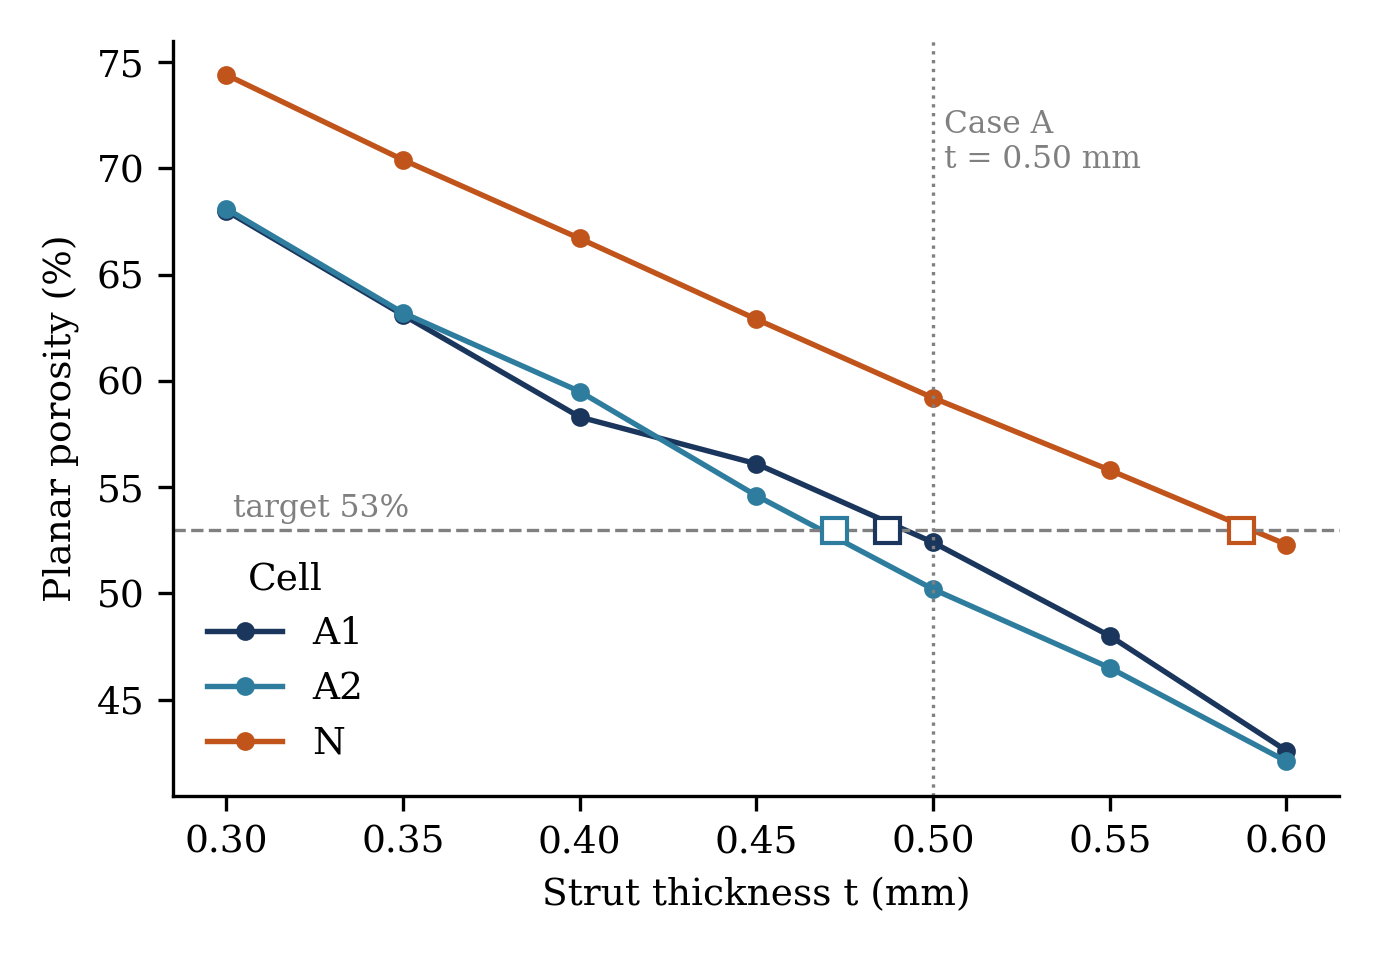
\includegraphics[width=\columnwidth]{figures/porosity.png}
\caption{Planar porosity against strut thickness for the three cells. Open squares mark the Case B thicknesses that give 53\% porosity. The dotted line marks Case A (t = 0.50 mm).}
\end{figure}
Third, the generator can vary the strut thickness along the screw axis. This is the lever for the collar hypothesis. With a graded thickness, the strut width grows from the core value $t_{c}$ to a denser value $t_{d}$ over a ramp of length $\ell$ next to the head:

\begin{equation}t(y) = t_c + (t_d - t_c)\,s(y)\end{equation}
where s(y) = min\{max[(y $-$ $Y_{h}$ + $\ell$) / $\ell$, 0], 1\} rises linearly from 0 to 1 over the ramp, and $Y_{h}$ is the axial position of the head end of the lattice. With $t_{d}$ = $t_{c}$, Equation 2 reduces to the uniform screw. We used $t_{c}$ = 0.472 mm (the Case B value for AS2), $t_{d}$ = 0.65 mm and $\ell$ = 6.0 mm. All design parameters sit in the model, so a graded screw needs one changed parameter and no new drawing. This is the practical benefit of the digital thread, and Section 6 shows it at work.

\subsection{The three cells}
The effective Poisson's ratio of the finished lattice is defined from the finite element strain field as

\begin{equation}\nu_{\mathrm{eff}} = -\,\frac{\varepsilon_{\mathrm{transverse}}}{\varepsilon_{\mathrm{axial}}}\end{equation}
The idealised hinge model of a honeycomb predicts a Poisson's ratio of +1 for a regular hexagon and a negative value for a re-entrant cell [21]. A finite-thickness lattice departs from that limit. A1 is a re-entrant chevron. Two vertical boundary struts, a central stem and two inward-sloping arms meet at an apex node. Axial tension pulls the arms outwards and pushes the walls apart, so the cell widens (reported $\nu_{\mathrm{eff}}$ = $-$0.22). The sharp apex hinges concentrate bending. A2 is a re-entrant hourglass built as an offset honeycomb with horizontal ribs and re-entrant waists. Its pores open under axial stretch, and it has the strongest auxetic response ($\nu_{\mathrm{eff}}$ = $-$0.41). We use the word chiral for A2 descriptively, because its strict chirality class has not been established [4]. N is a conventional hexagon with outward diagonals at 120\textdegree{}. It contracts sideways under tension ($\nu_{\mathrm{eff}}$ = +0.31) and serves as the control. The three $\nu_{\mathrm{eff}}$ values come from the project's unit-cell finite element dataset and were not recomputed here.


\section{Verification by Simulation}
\subsection{Finite element model}
Each screw was analysed in COMSOL Multiphysics 6.2 as a displacement-controlled axial tensile test of the isolated screw. The STEP geometry from Fusion 360 was imported and merged into one solid with a repair tolerance of 10\textbackslash{}textsuperscript\{\$-\$5\} m. All displacement components were fixed on the faces of the conical tip, and an axial displacement $U_{y}$ = +0.20 mm ($U_{x}$ = $U_{z}$ = 0) was prescribed on the faces of the head. The boundary faces were picked by coordinate boxes, so the same rule applies to every screw. All three screws have a strut thickness of 0.50 mm (Case A), so their porosities are 52.4\% (AS1), 50.2\% (AS2) and 59.2\% (NS). The material was Ti-6Al-4V ELI, treated as isotropic and linear elastic (Table 3). The mesh used quadratic tetrahedra, and the system was solved with the PARDISO direct solver. Each run took a few minutes on a 12-core workstation with 32 GB of memory. The axial stiffness follows from the reaction force:

\begin{equation}K = \frac{F_y}{U_y}\end{equation}
\begin{table}[!t]
\caption{Material properties used in the model, with the specified minima for wrought Ti-6Al-4V ELI.}
\centering\fontsize{8}{9.6}\selectfont
\begin{tabular}{>{\raggedright\arraybackslash}p{\dimexpr(\linewidth-6\tabcolsep)*323/1000\relax}>{\centering\arraybackslash}p{\dimexpr(\linewidth-6\tabcolsep)*258/1000\relax}>{\centering\arraybackslash}p{\dimexpr(\linewidth-6\tabcolsep)*419/1000\relax}}
\toprule
\textbf{Property} & \textbf{Value in model} & \textbf{Specified minimum (wrought, ASTM F136)} \\
\midrule
\textbf{Young's modulus E} & 110 GPa & not specified \\
\textbf{Poisson's ratio $\nu$} & 0.33 & not specified \\
\textbf{Yield strength $\sigma_{y}$ (0.2\%)} & 850 MPa & 795 MPa \\
\textbf{Ultimate strength $\sigma_{\mathrm{uts}}$} & 960 MPa & 860 MPa \\
\bottomrule
\end{tabular}
\par\vspace{3pt}{\raggedright\fontsize{7.5}{9}\selectfont\itshape The model values for yield and ultimate strength are typical values. SLM-built lattices must be tested because their properties depend on process, build direction and post-processing [22].\par}
\end{table}
The model has no bone, no contact or friction, no insertion preload and no cyclic load. The reaction force is therefore the force needed to stretch the screw by 0.20 mm. It measures the axial stiffness of the structure. It is not the pullout force of a screw in bone, and by Equation 4 it carries the same information as K. We call it the axial reaction force in the rest of the paper.

\subsection{Mesh convergence}
Our first runs used a single mesh (COMSOL size level 6, called Coarse). This is not enough to judge a result, so we repeated every screw on five levels, from level 7 (Coarser) to level 3 (Finer). The mesh grew from about 23,000 to about 300,000 elements. Table 4 and Figure 4 give the results.

\begin{table*}[!t]
\caption{Mesh study. Axial reaction force $F_{y}$ at the original mesh (level 6) and the finest mesh (level 3), stiffness on the finest mesh, and peak von Mises stress.}
\centering\fontsize{8}{9.6}\selectfont
\begin{tabular}{>{\raggedright\arraybackslash}p{\dimexpr(\linewidth-16\tabcolsep)*125/1000\relax}>{\centering\arraybackslash}p{\dimexpr(\linewidth-16\tabcolsep)*125/1000\relax}>{\centering\arraybackslash}p{\dimexpr(\linewidth-16\tabcolsep)*125/1000\relax}>{\centering\arraybackslash}p{\dimexpr(\linewidth-16\tabcolsep)*125/1000\relax}>{\centering\arraybackslash}p{\dimexpr(\linewidth-16\tabcolsep)*125/1000\relax}>{\centering\arraybackslash}p{\dimexpr(\linewidth-16\tabcolsep)*125/1000\relax}>{\centering\arraybackslash}p{\dimexpr(\linewidth-16\tabcolsep)*125/1000\relax}>{\centering\arraybackslash}p{\dimexpr(\linewidth-16\tabcolsep)*125/1000\relax}}
\toprule
\textbf{Screw} & \textbf{$F_{y}$ level 6 (N)} & \textbf{$F_{y}$ level 3 (N)} & \textbf{Change} & \textbf{K level 3 (kN/mm)} & \textbf{Peak $\sigma$ level 6 (MPa)} & \textbf{Peak $\sigma$ level 3 (MPa)} & \textbf{Collar-zone $\sigma$ level 3 (MPa)} \\
\midrule
\textbf{AS1 (chevron)} & 3,128.2 & 3,096.2 & -1.0\% & 15.48 & 11,163 & 17,146 & 11,401 \\
\textbf{AS2 (hourglass)} & 2,437.6 & 2,382.1 & -2.3\% & 11.91 & 5,101 & 6,312 & 6,312 \\
\textbf{NS (hexagon)} & 1,009.0 & 957.9 & -5.1\% & 4.79 & 4,196 & 4,099 & 1,592 \\
\bottomrule
\end{tabular}
\par\vspace{3pt}{\raggedright\fontsize{7.5}{9}\selectfont\itshape Collar zone: axial window 24.0 to 26.5 mm, which contains the last lattice row, the collar and the taper.\par}
\end{table*}
\begin{figure*}[!t]
\centering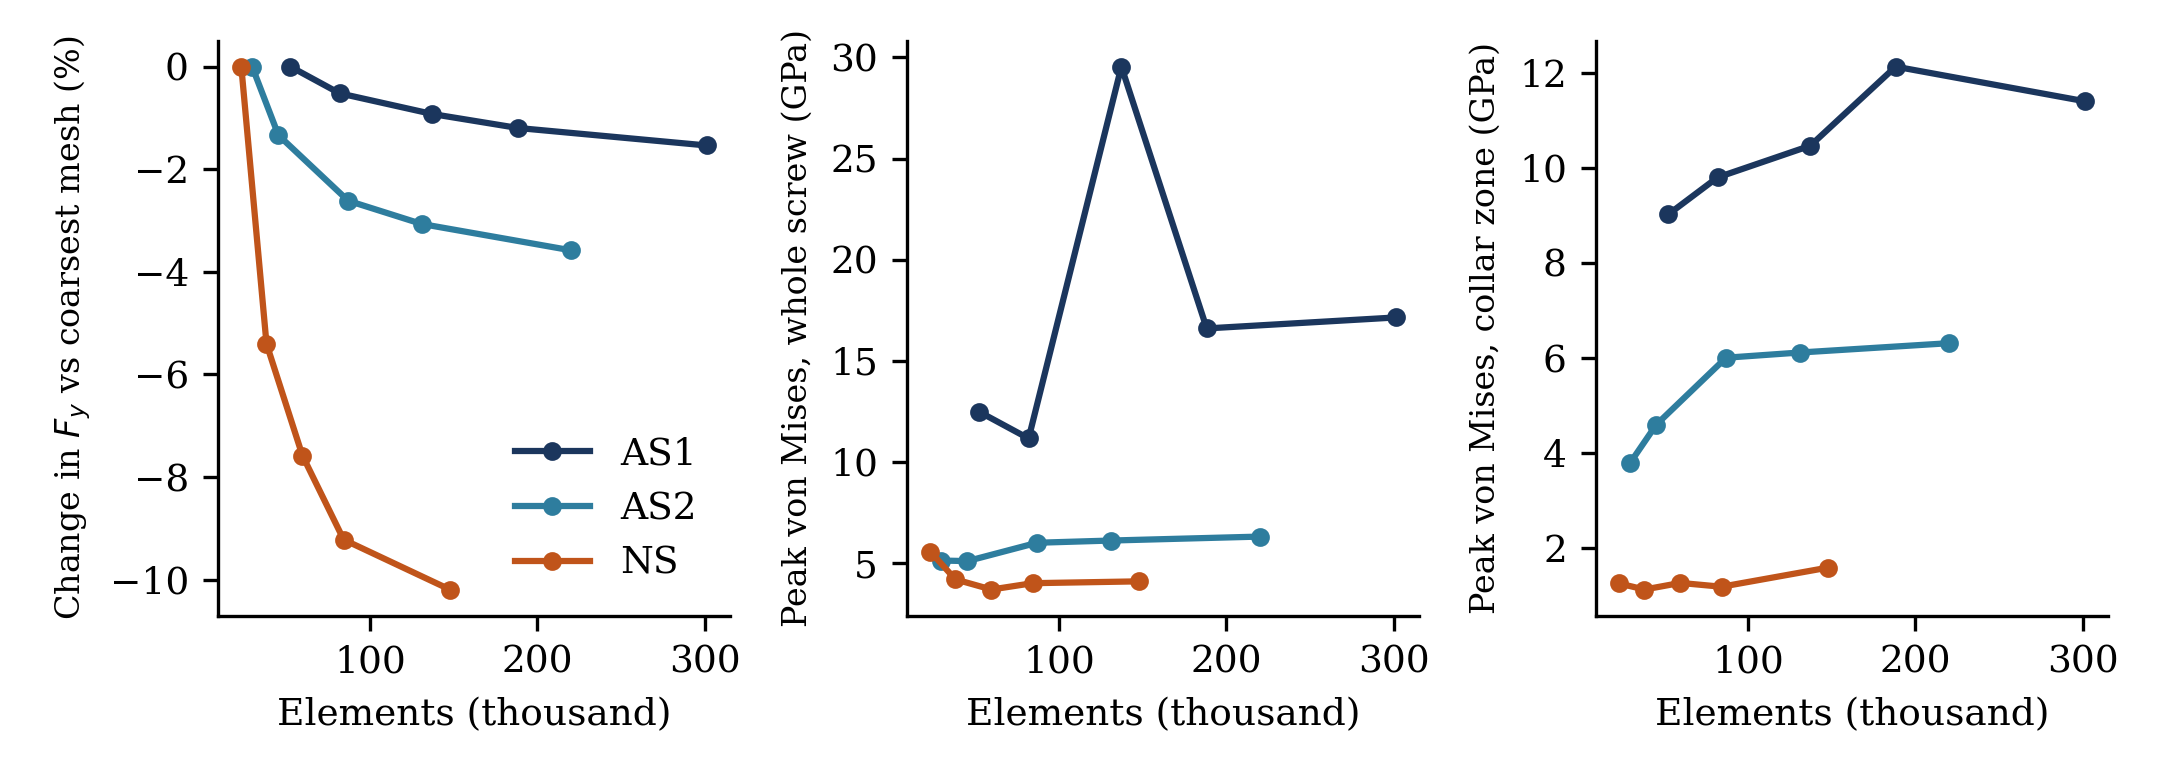
\includegraphics[width=\textwidth]{figures/convergence.png}
\caption{Mesh study for the three screws. (a) Change in axial reaction force relative to the coarsest mesh. (b) Peak von Mises stress over the whole screw. (c) Peak von Mises stress in the collar zone.}
\end{figure*}
The force behaves well. It falls steadily as the mesh is refined, by 1.5\% for AS1, 3.6\% for AS2 and 10.2\% for NS between the coarsest and the finest mesh. The drop between levels 4 and 3 is only 0.3\%, 0.5\% and 1.1\%, so the values are close to settled. The results are presented with the finest-mesh numbers, AS1 3,096 N, AS2 2,382 N and NS 958 N, together with the original level-6 numbers. The ordering AS1 > AS2 > NS is the same on every mesh.

The stress does not behave. The whole-screw peak for AS1 jumps between 11 and 30 GPa and never settles, and AS2 and NS drift upwards or sideways. This is the behaviour expected from a stress singularity, a sharp corner where linear elasticity predicts a stress that grows without bound as the mesh is refined. The stress values are also far above the yield strength, 850 MPa, by a factor of 4 to more than 20. A linear-elastic stress above yield has no direct physical meaning, because a real screw would yield and redistribute the load. We therefore do not report any peak stress as a prediction of safety. We use the stress only to rank the topologies, and only where the ranking is stable.

The collar-zone stress is more useful. It rises slowly with refinement but keeps the same ordering on every mesh from level 6 to level 3: AS1 (9,800 to 12,100 MPa), then AS2 (4,600 to 6,300 MPa), then NS (about 1,100 to 1,600 MPa). For AS2 the whole-screw peak lies inside this window on all three finest meshes. For this screw the highest stress is therefore found at the transition between lattice and head, which agrees with the location reported for fatigue failure in [9]. The window also contains the end of the lattice, so this result cannot separate the collar from the lattice end.

\subsection{Force, stiffness and the fixation hypothesis}
On the finest mesh AS1 carries 3.23 times the force of NS and AS2 carries 2.49 times (for the original mesh the ratios are 3.10 and 2.42). AS2 keeps 77\% of the AS1 force. The stiffnesses are 15.5, 11.9 and 4.8 kN/mm. Force and stiffness are one result written twice, because the displacement is the same for all screws, and they should not be counted as separate evidence.

AS2 is the more strongly auxetic design ($\nu_{\mathrm{eff}}$ = $-$0.41 against $-$0.22), yet AS1 carries more force. In this dataset the force follows the axial stiffness and not the size of $\nu_{\mathrm{eff}}$. There is no bone in the model, so radial expansion creates no contact pressure, and the idea that auxetic expansion improves grip is neither tested nor confirmed. Yao et al. found that the benefit of stronger auxeticity appears at matched modulus [6], while Barnett et al. found that low stiffness can also help [1]. AS1 and AS2 differ in both stiffness and $\nu_{\mathrm{eff}}$, so their effects cannot be separated here.

The requirement FR-02 also needs a second look. Its limit of 1,000 N is almost exactly the response of the control: NS gave 1,009 N on the original mesh and only 958 N on the finest one. A limit set at the control's own value cannot tell an auxetic screw from a conventional one. We recommend rewriting FR-02 as a pullout requirement in a bone analogue, stated relative to a non-auxetic control of equal porosity. Section 6 carries this change into the trace.

The comparison with NS is not at equal porosity. NS is more porous (59.2\%) and is also the weakest screw. At the same porosity it would be stiffer, so the force ratios above probably overstate the advantage of the auxetic cells. Simulating the Case B geometries would remove this confounding and is the first item of future work. A check on stiffness is useful. A fully solid annular shaft with the S3 dimensions (cross-section 16.96 mm\textsuperscript{2}) and E = 110 GPa would have EA/L of about 89 kN/mm. The lattice screws are 6 to 19 times more compliant than this. Whether that compliance reduces stress shielding depends on the stiffness of the bone, and our model does not include bone, so we make no claim about shielding.


\section{Graded Transition Study}
The collar hypothesis says that a smoother change in stiffness between the lattice and the head should relieve the transition. We tested one version of this idea with the generative design step of Section 4.3. A uniform AS2 screw (AS2U, t = 0.472 mm) was compared with a graded AS2 screw (AS2G) whose strut thickness rises linearly from 0.472 mm to 0.65 mm over the last 6.0 mm of the lattice (Equation 2 and Figure 5a). The two screws came from the same Fusion 360 script. Only the parameter GRADE\_ON differed, so the comparison is clean. The loading, the boundary conditions and the four finest mesh levels (6 to 3) were the same as in Section 5.

The grading adds little material. The screw volume rises from 339.6 to 343.6 mm\textsuperscript{3}, which is 1.2\%. The results are in Table 5 and Figure 5. We report the finest mesh first and then say how the other meshes agree.

\begin{table}[!t]
\caption{Uniform (AS2U) and graded (AS2G) screws on the finest mesh (level 3), and the change due to grading.}
\centering\fontsize{8}{9.6}\selectfont
\begin{tabular}{>{\raggedright\arraybackslash}p{\dimexpr(\linewidth-8\tabcolsep)*508/1000\relax}>{\centering\arraybackslash}p{\dimexpr(\linewidth-8\tabcolsep)*169/1000\relax}>{\centering\arraybackslash}p{\dimexpr(\linewidth-8\tabcolsep)*169/1000\relax}>{\centering\arraybackslash}p{\dimexpr(\linewidth-8\tabcolsep)*153/1000\relax}}
\toprule
\textbf{Quantity} & \textbf{AS2U} & \textbf{AS2G} & \textbf{Change} \\
\midrule
\textbf{Axial reaction force $F_{y}$ (N)} & 2,224 & 2,341 & +5.3\% \\
\textbf{Collar-zone peak stress, 24--26.5 mm (MPa)} & 6,428 & 5,229 & $-$18.7\% \\
\textbf{Ramp-zone peak stress, 19--24 mm (MPa)} & 6,116 & 7,770 & +27.0\% \\
\textbf{Whole-screw peak stress (MPa)} & 6,932 & 7,770 & +12.1\% \\
\textbf{Screw volume (mm\textsuperscript{3})} & 339.6 & 343.6 & +1.2\% \\
\bottomrule
\end{tabular}
\par\vspace{3pt}{\raggedright\fontsize{7.5}{9}\selectfont\itshape All stresses are linear-elastic peaks and are used for comparison only.\par}
\end{table}
\begin{figure*}[!t]
\centering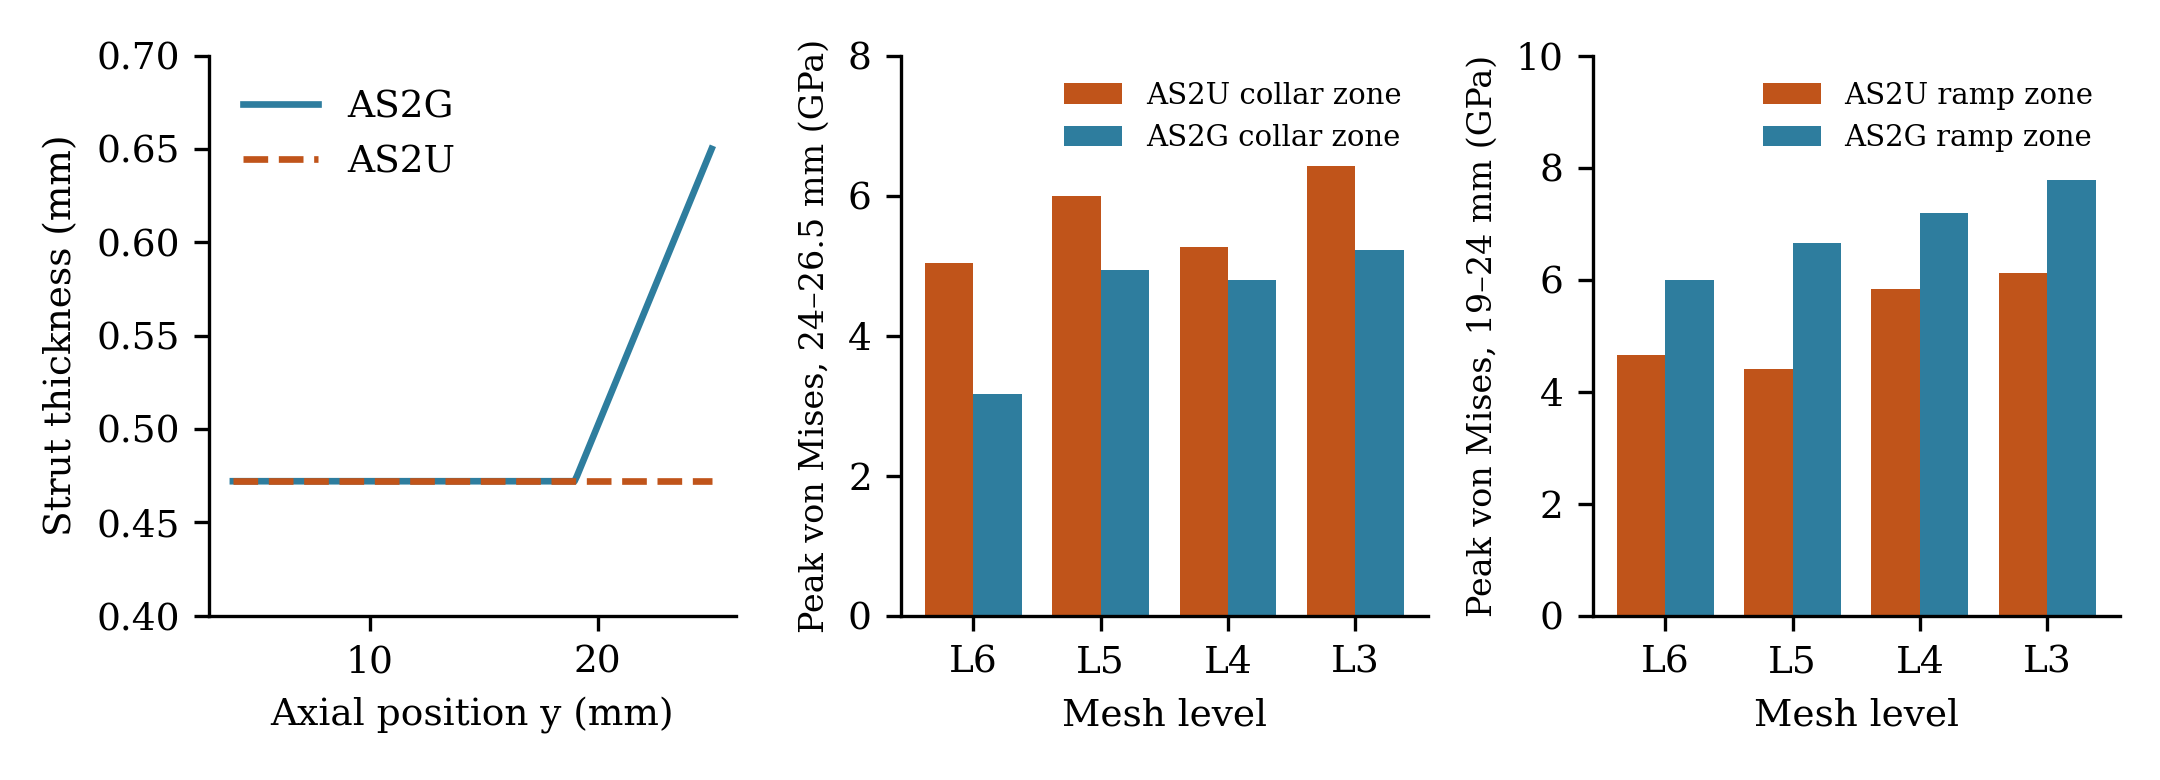
\includegraphics[width=\textwidth]{figures/graded.png}
\caption{Graded transition study. (a) Strut thickness along the screw axis for AS2G (graded) and AS2U (uniform). (b) Peak von Mises stress in the collar zone. (c) Peak von Mises stress in the ramp zone. L6 to L3 are the four mesh levels, from coarse to fine.}
\end{figure*}
Grading did what it was designed to do next to the head. The collar-zone stress is lower on every mesh, by 37\%, 18\%, 9\% and 19\% from level 6 to level 3. The axial force also rises by about 5\% on every mesh. Grading also had a cost. The peak stress in the ramp zone is higher on every mesh, by 29\%, 51\%, 24\% and 27\%, and on the two finest meshes the whole-screw peak of AS2G lies in this zone. The hot spot has moved from the head end of the lattice to the place where the thick and thin struts meet.

The result is negative but informative. It supports a cautious reading of the transition paradox: a stiffness step cannot be removed by moving it. A linear ramp over 6 mm still has an abrupt change in strut thickness at its start, and that change collects stress. The result does not show that grading is a bad idea. Longer or curved ramps and node fillets are the next things to try, and the model makes each of them a one-parameter change. The comparison also says nothing about fatigue life. It shows that the collar hypothesis cannot be confirmed or rejected by comparing linear peak stresses. A fatigue-based criterion, measured on as-built SLM lattices, is needed.

The uniform control also gives a sensitivity check on the baseline. AS2U (t = 0.472 mm) carries 2,224 N and AS2 from Section 5 (t = 0.50 mm) carries 2,382 N on the finest mesh. A 5.6\% thinner strut therefore costs 6.6\% of the force. The force depends on strut thickness almost in proportion, so a Case B comparison at equal porosity will change the numbers in Table 4 by several per cent.


\section{Requirements Traceability}
A trace link and the evidence behind it are two different things. A link is a property of the model: it shows that a requirement has an owner, a design parameter and a verification case. Evidence is a property of the results: it shows whether the requirement was met. Table 6 records both. All eight requirements are linked. The simulations support FR-01, FR-04, NFR-02 and the strut-thickness part of NFR-03. They support FR-02 only in part. FR-03 and NFR-01 remain open. NFR-04 is met at link level only.

\begin{table*}[!t]
\caption{Traceability from requirement to verification case and evidence status.}
\centering\fontsize{8}{9.6}\selectfont
\begin{tabular}{>{\raggedright\arraybackslash}p{\dimexpr(\linewidth-10\tabcolsep)*92/1000\relax}>{\centering\arraybackslash}p{\dimexpr(\linewidth-10\tabcolsep)*231/1000\relax}>{\raggedright\arraybackslash}p{\dimexpr(\linewidth-10\tabcolsep)*262/1000\relax}>{\centering\arraybackslash}p{\dimexpr(\linewidth-10\tabcolsep)*200/1000\relax}>{\raggedright\arraybackslash}p{\dimexpr(\linewidth-10\tabcolsep)*215/1000\relax}}
\toprule
\textbf{Req.} & \textbf{Design parameter / block} & \textbf{Verification case} & \textbf{Result} & \textbf{Status} \\
\midrule
\textbf{FR-01} & Cell topology, S3 & Unit-cell FE, $\nu_{\mathrm{eff}}$ & $-$0.22, $-$0.41, +0.31 & Met (AS1, AS2) \\
\textbf{FR-02} & Whole screw, S4 & Axial tension, $F_{y}$ at 0.20 mm & 3,096 / 2,382 / 958 N & Partial: no bone; limit must be reset \\
\textbf{FR-03} & S1, S2 & Torsion model & not run & Open \\
\textbf{FR-04} & Strut thickness t, S3 & CAD porosity, Eq. 1 & 52.4 / 50.2 / 59.2\% & Met for AS1, AS2; NS above window \\
\textbf{NFR-01} & Collar geometry, S2 & Collar-zone stress, Sections 5.2 and 6 & Stress not converged & Open: linear stress above yield \\
\textbf{NFR-02} & D1, L, P in CAD & Dimension check in CAD & 5.70 / 21.0 / 1.75 mm & Met by construction \\
\textbf{NFR-03} & Strut thickness, S3 & Parameter check & 0.50 / 0.50 / 0.50 mm & Met for t; pore size not checked \\
\textbf{NFR-04} & System model & Link audit & 8 of 8 linked & Met at link level \\
\bottomrule
\end{tabular}
\par\vspace{3pt}{\raggedright\fontsize{7.5}{9}\selectfont\itshape The three results in order are AS1, AS2 and NS. FR-04 and NFR-03 use the Case A geometry that was simulated.\par}
\end{table*}
To keep the claims honest, we use four evidence levels. Level E1 is simulated verification, in which a design output is checked against a requirement by computation. This is partly reached. Level E2 is physical verification, which means bench tests of manufactured screws, for example by ASTM F543 methods [23]. Level E3 is validation, which shows that the device meets user needs in realistic conditions. Level E4 is regulatory acceptance. Only E1 is present in this paper. Under ISO 13485 [15] the matching records are planning (7.3.2), inputs (7.3.3), outputs (7.3.4), review (7.3.5), verification (7.3.6), validation (7.3.7), transfer (7.3.8), change control (7.3.9) and the design and development file (7.3.10). This paper is not a regulatory submission.


\section{Discussion}
\subsection{What the framework gave us}
We return to the three research questions. For RQ1, the answer is yes. All geometry came from a parameter set in the model, and two new variants (the uniform control and the graded screw) needed one changed parameter each. The same applies to the mesh study, where the same batch script was run at five levels. This is the practical benefit of a digital thread: a question that would normally need a day of redrawing took one script change.

For RQ2, a simulation-only verification can rank the topologies by stiffness, and it can show whether a requirement is plausible. It cannot say anything about fixation in bone, fatigue life or safety. The unconverged stress is the clearest example. A single-mesh run gave a precise-looking number, 11,163 MPa for AS1, and the mesh study showed that this number had no meaning. A systems engineer who only checks whether a requirement has a linked simulation would have marked it as verified.

For RQ3, the trace was useful in four places. First, writing FR-02 into the model showed that its limit of 1,000 N equals the control's own response, so it cannot separate auxetic from conventional screws. Second, listing the verification case of NFR-01 showed that no result addressed the collar neck. This led to the collar-zone measure and to the graded study. Third, separating a link from its evidence made it clear that NFR-04 (traceability) had been met only formally. Fourth, tracing the geometry parameters back to their generating script exposed the strut-thickness question of Section 5. The finite element geometry came from a script with a fixed thickness of 0.50 mm, and not from the porosity-calibrated 0.472 to 0.587 mm values of Case B. An audit trail that was only a document would not have caught this.

\subsection{Lessons for systems engineering practice}
Four lessons carry over to other projects. Acceptance criteria must be able to discriminate: a limit equal to the control's response is not a requirement, and fixation targets should be stated relative to a baseline design. Each trace link should also carry its evidence level, because a link only says that a check exists, while the level says what the check can prove. Simulated, bench, validation and regulatory evidence should not share one status column. Third, the model should be verified before the design is. A mesh study checks the verification method itself and belongs in the model as a standard case. Finally, the generator should be versioned with the geometry. A STEP file without the script and parameter values that made it cannot be traced, and the porosity calibration and the simulated geometry must refer to the same parameters.

\subsection{Limitations}
The study has several limits. The simulations are linear elastic with one load case, no bone and no cyclic loading. Peak stresses are not converged and cannot be read as physical values. The finite element results are for the equal-thickness geometry (Case A) and do not give an equal-porosity comparison. The effective Poisson's ratios are from an earlier dataset and were not recomputed. Porosity is a planar value, and its relation to the volume porosity of the wrapped lattice is unknown. Material data are typical wrought values and not measured as-built SLM values. The A1 calibration entry is about one point inconsistent with the porosity curve. The 1.5 N$\cdot$m torque limit (FR-03) and the safety factor of 1.5 (NFR-01) are design assumptions and are not taken from a standard. The effect of the collar on fatigue is a hypothesis. We did not search the literature in a systematic way.

\subsection{Future work}
The next steps are, in order: (1) simulate the Case B geometries for an equal-porosity comparison; (2) add fillets at the strut junctions, within SLM limits, and use elastoplastic material and geometric nonlinearity; (3) sweep the ramp length and shape and add a no-collar baseline; (4) measure as-built material properties and run tensile and torsion tests on printed screws; (5) run ASTM F543 pullout tests in a bone analogue [23]; and (6) build a bone-contact model and carry out fatigue tests. Steps 4 to 6 would move the evidence from level E1 to E2 and E3. The assumed torque limit should be replaced by the ASTM F543 requirement once the standard has been obtained and the screw has been tested.


\section{Conclusions}
This paper presented an MBSE framework for auxetic bone screws. SysML requirements, a four-subsystem architecture, a requirements-driven generative design step and a COMSOL workflow are connected by an explicit trace. Four conclusions follow.

\begin{itemize}
\item[\textbf{(1)}] On the finest mesh, and for equal strut thickness, the AS1, AS2 and NS screws gave axial reaction forces of 3,096, 2,382 and 958 N under a 0.20 mm displacement. The force changed by 1.5\% to 10\% over the mesh study. This is a stiffness result for the isolated screw and not evidence of better fixation in bone.
\item[\textbf{(2)}] Peak von Mises stress did not converge and was 4 to more than 20 times the yield strength. It was used only to rank the screws. The collar-zone ranking AS1 > AS2 > NS was stable on every mesh.
\item[\textbf{(3)}] Grading the strut thickness over a 6 mm ramp lowered the collar-zone stress by about 19\% and raised the force by 5\%, but moved the stress hot spot into the ramp. The stiffness step was moved and not removed.
\item[\textbf{(4)}] All eight requirements are linked, but the evidence is simulated, and FR-03 and NFR-01 are open. The trace exposed a weak acceptance criterion (FR-02), a missing check at the collar neck and a geometry-provenance gap.
\end{itemize}
For systems engineers, the main point is that a model-based trace is most valuable when it shows what the evidence cannot prove. Physical testing and a bone-contact model are the necessary next steps before any fixation or fatigue claim can be made.

\begingroup\footnotesize\setlength{\parskip}{1.5pt}
\begin{thebibliography}{99}
\setlength{\itemsep}{1.5pt}
\bibitem{r1} Barnett E, Fletcher J, Gill HS, Pegg EC, Loukaides EG. Auxetic fixation devices can achieve superior pullout performances compared to standard fixation concepts. Smart Mater Struct. 2024;33(6):065010. doi:10.1088/1361-665X/ad442d
\bibitem{r2} Yao Y, Wang L, Li J, Tian S, Zhang M, Fan Y. A novel auxetic structure based bone screw design: Tensile mechanical characterization and pullout fixation strength evaluation. Mater Des. 2020;188:108424. doi:10.1016/j.matdes.2019.108424
\bibitem{r3} Lakes R. Foam structures with a negative Poisson's ratio. Science. 1987;235(4792):1038-1040. doi:10.1126/science.235.4792.1038
\bibitem{r4} Kelkar PU, Kim HS, Cho K-H, Kwak JY, Kang C-Y, Song H-C. Cellular auxetic structures for mechanical metamaterials: a review. Sensors. 2020;20(11):3132. doi:10.3390/s20113132
\bibitem{r5} Sun M, Hu X, Tian L, Yang X, Min L. Auxetic biomedical metamaterials for orthopedic surgery applications: a comprehensive review. Orthop Surg. 2024;16(8):1801-1815. doi:10.1111/os.14142
\bibitem{r6} Yao Y, Yuan H, Huang H, Liu J, Wang L, Fan Y. Biomechanical design and analysis of auxetic pedicle screw to resist loosening. Comput Biol Med. 2021;133:104386. doi:10.1016/j.compbiomed.2021.104386
\bibitem{r7} Wang L, Huang H, Yuan H, et al. In vitro fatigue behavior and in vivo osseointegration of the auxetic porous bone screw. Acta Biomater. 2023;170:185-201. doi:10.1016/j.actbio.2023.08.040
\bibitem{r8} Huang H, Liu J, Yao Y, Wang L, Fan Y. Stress concentration in the auxetic porous screw and its fatigue behavior. Compos Struct. 2024;345:118403. doi:10.1016/j.compstruct.2024.118403
\bibitem{r9} Huang H, Liu J, Yao Y, Wang L, Fan Y. Fatigue behavior of the auxetic porous bone screw under the multiaxial cyclic loads in tibiotalocalcaneal arthrodesis. Ann Biomed Eng. 2025;53(5):1113-1127. doi:10.1007/s10439-025-03693-3
\bibitem{r10} Madni AM, Sievers M. Model-based systems engineering: motivation, current status, and research opportunities. Syst Eng. 2018;21(3):172-190. doi:10.1002/sys.21438
\bibitem{r11} INCOSE. Systems Engineering Handbook: A Guide for System Life Cycle Processes and Activities. 5th ed. Walden DD, Shortell TM, Roedler GJ, et al., eds. Hoboken, NJ: John Wiley \& Sons; 2023. ISBN 978-1-119-81429-0
\bibitem{r12} ISO/IEC/IEEE 15288:2023. Systems and software engineering --- System life cycle processes. Geneva: International Organization for Standardization; 2023.
\bibitem{r13} Friedenthal S, Moore A, Steiner R. A Practical Guide to SysML: The Systems Modeling Language. 3rd ed. Waltham, MA: Morgan Kaufmann/OMG Press; 2014.
\bibitem{r14} Object Management Group. OMG Systems Modeling Language (SysML), Version 2.0. Needham, MA: OMG; 2025 (final adoption approved July 2025). \url{https://www.omg.org/spec/SysML/2.0}
\bibitem{r15} ISO 13485:2016. Medical devices --- Quality management systems --- Requirements for regulatory purposes. Geneva: International Organization for Standardization; 2016.
\bibitem{r16} U.S. Food and Drug Administration. Medical devices; Quality System Regulation amendments (Quality Management System Regulation, QMSR), final rule. Fed Regist. 2024;89:7496 (published 2 February 2024; effective 2 February 2026).
\bibitem{r17} U.S. Code of Federal Regulations. Title 21, Part 820 --- Quality Management System Regulation, as amended effective 2 February 2026 (incorporating ISO 13485:2016 by reference).
\bibitem{r18} ISO 14971:2019. Medical devices --- Application of risk management to medical devices. Geneva: International Organization for Standardization; 2019.
\bibitem{r19} ASME V\&V 40-2018. Assessing Credibility of Computational Modeling through Verification and Validation: Application to Medical Devices. New York: American Society of Mechanical Engineers; 2018.
\bibitem{r20} U.S. Food and Drug Administration. Assessing the Credibility of Computational Modeling and Simulation in Medical Device Submissions: Guidance for Industry and FDA Staff. Final guidance issued 16 November 2023.
\bibitem{r21} Gibson LJ, Ashby MF. Cellular Solids: Structure and Properties. 2nd ed. Cambridge University Press; 1997. doi:10.1017/CBO9781139878326
\bibitem{r22} ASTM International. ASTM F136: Standard Specification for Wrought Titanium-6Aluminum-4Vanadium ELI (Extra Low Interstitial) Alloy for Surgical Implant Applications (UNS R56401). West Conshohocken, PA: ASTM International (current edition; specified minima quoted: Rp0.2 $\geq$ 795 MPa, Rm $\geq$ 860 MPa).
\bibitem{r23} ASTM International. ASTM F543-23: Standard Specification and Test Methods for Metallic Medical Bone Screws. West Conshohocken, PA: ASTM International; 2023 (supersedes F543-17). doi:10.1520/F0543-23
\bibitem{r24} U.S. Food and Drug Administration. Orthopedic Non-Spinal Metallic Bone Screws and Washers: Performance Criteria for Safety and Performance Based Pathway. Guidance for Industry and FDA Staff (issued as draft, 2019; docket FDA-2019-D-1652). \url{https://www.fda.gov/regulatory-information/search-fda-guidance-documents/orthopedic-non-spinal-metallic-bone-screws-and-washers-performance-criteria-safety-and-performance}
\end{thebibliography}
\endgroup

\end{document}
